% JUMP TO LINE 60, 75
\documentclass{article}
\usepackage[letterpaper,portrait,top=0.4in, left=0.6in, right=0.6in, bottom=1in]{geometry}

\usepackage{amsmath, amsfonts, amsthm, amssymb}
\usepackage{graphicx, float}
\usepackage{mathtools}
\usepackage{titlesec}
\usepackage{interval}
\usepackage{hyperref}
\usepackage{siunitx}
\usepackage{titling}
\usepackage{pdfpages}
\usepackage{vwcol}
\usepackage{setspace}
\usepackage{empheq}
\usepackage{cancel}
\usepackage{esdiff}
\usepackage{multicol}
\usepackage{mdframed}
\usepackage{esdiff}
\usepackage{tikzsymbols}
\usepackage{multicol}
\usepackage{tikz}
\usepackage{varwidth}
\usepackage{parskip}
\usepackage{pgfplots}
\usepackage{mlmodern}
\pgfplotsset{compat=1.18}
\intervalconfig {
	soft open fences
}

\newcommand{\alignedintertext}[1]{%
  \noalign{%
    \vtop{\hsize=\linewidth#1\par
    \expandafter}%
    \expandafter\prevdepth\the\prevdepth
  }%
}

\newtheorem{lemma}{Lemma}

\newcommand*{\problem}[1]{\section*{Problem #1}}
\newcommand*{\aps}{\section*{AP Corner}}
\newcommand*{\deriv}[1][x]{\ensuremath{\dfrac{\mathrm{d}}{\mathrm{d}#1}}}
\newcommand*{\floor}[1]{\ensuremath{\lfloor #1\rfloor}}
\newcommand*{\lheqzero}{\ensuremath{\underset{\text{L'H}}{\overset{\left[\frac00\right]}{=}}}}
\newcommand*{\lheqinfty}{\ensuremath{\underset{\text{L'H}}{\overset{\left[\frac{\infty}{\infty}\right]}{=}}}}

\DeclareMathOperator{\DNE}{DNE}
\DeclareMathOperator{\sgn}{sgn}

\DeclareMathOperator{\arccsc}{arccsc}
\DeclareMathOperator{\arcsec}{arcsec}
\DeclareMathOperator{\arccot}{arccot}

%opening

\postdisplaypenalty=100000

\begin{document}
\setstretch{1.25}
\fontsize{12pt}{12pt}\selectfont
\setlength{\abovedisplayskip}{\abovedisplayskip/2}
\setlength{\belowdisplayskip}{\belowdisplayskip/2}
\setlength{\parindent}{0pt}
\setlength{\parskip}{2ex plus 0.5ex minus 0.2ex}

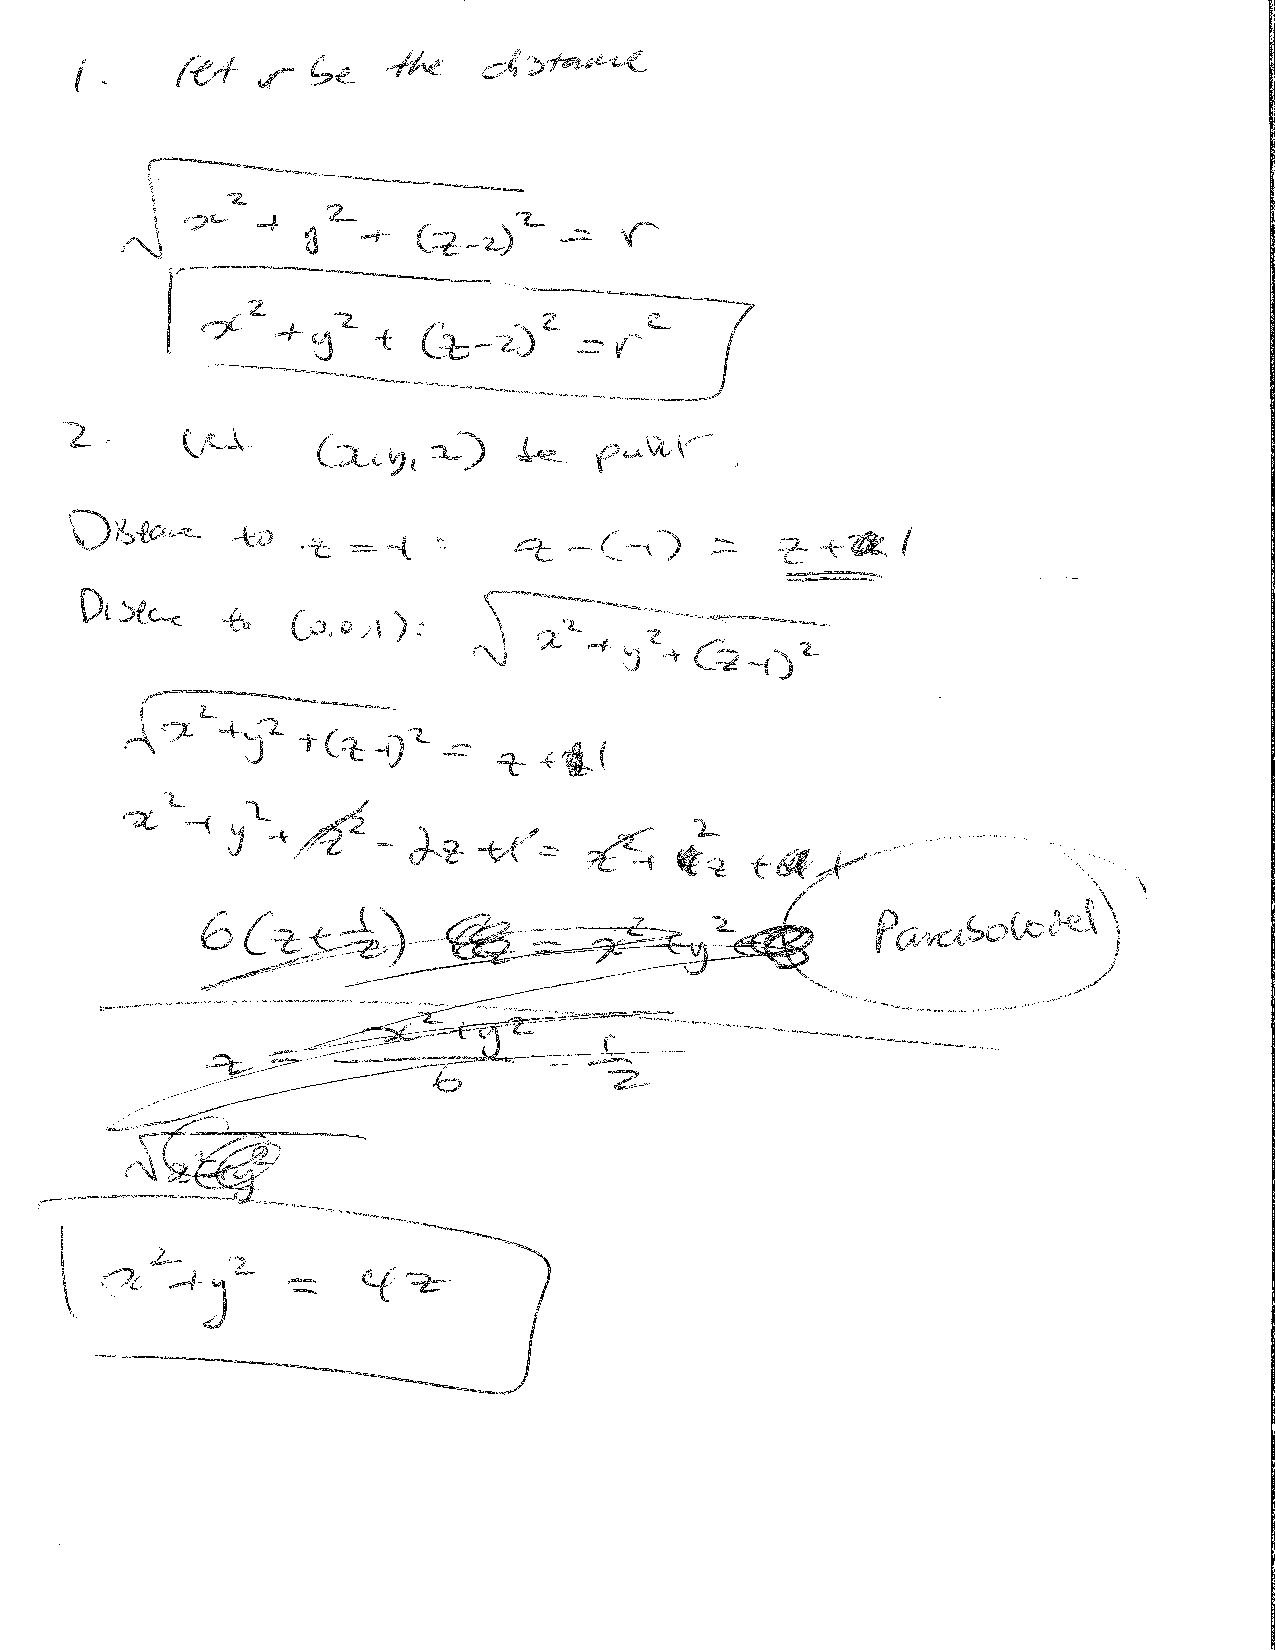
\includepdf[pages=-]{q1.4.pdf}

\problem{4}

\begin{itemize}
\item[(b)]
	Solid of revolution created by revolving $y=4x-x^2$ about the $x$-axis. We evaluate the volume between $x=0$ and $x=4$.

	$\begin{aligned}[t]
		V
		&=\int_{0}^{4}\pi r^2\,\mathrm{d}x
		=\pi\int_{0}^{4}\left( 4x-x^2 \right)^2\mathrm{d}x
		=\pi \int_{0}^{4}\left( 16x^2-8x^3+x^4 \right)\mathrm{d}x
		=\pi\left[\frac{16x^3}{3}-\frac{8x^4}{4}+\frac{x^5}{5}\right]_{0}^{4}\\
		&=\pi\left(\frac{16(4)^3}{3}-2(4)^4+\frac{4^5}{5}\right)
		=\pi\left(\frac{1024}{3}-512+\frac{1024}{5}\right)
		=\pi \left( \frac{5120-7680+3072}{15} \right)
		=\boxed{\frac{512\pi}{15}}
	\end{aligned}$
\end{itemize}

\problem{5}
\begin{itemize}
\item[(a)] Solid of revolution formed by rotating $y=\sin z$ about the $z$ axis. Oscillation is in the vertical ($z$) direction. The traces of the solid parallel to the $xy$-plane are circles with radius $(\sin z)$.

\item[(b)] Same as before, in that the traces parallel to the $xy$-plane are circles, but they are of radius $\sqrt{\sin z}$, which is only real if $\sin z\geq0 \iff 2\pi k\leq z\leq \pi+2\pi k$ where $k\in\mathbb Z$.

For values of $z$ satisfying $2\pi k\leq z\leq \pi+2\pi k$ where $k\in\mathbb Z$, the trace of the solid parallel to the $xy$-plane is a circle of radius $\sqrt{\sin z}$. For $z$-values not satisfying the inequality, the trace at that $z$ value is empty.

The solid is a collection of discontinuous ``bulbs'' that occur every $2\pi$ units in the $z$-direction.

\end{itemize}

\end{document}
